%!TEX TS-program = xelatex

%Pacotes e preâmbulo 
\documentclass[a4paper, 14pt, twoside]{article}
\usepackage{graphicx}
\usepackage[brazil]{babel}
\usepackage[lmargin=3cm,tmargin=3cm,rmargin=2cm,bmargin=2cm]{geometry}
\usepackage{fontspec}
\usepackage{amsmath,amsthm,amsfonts,amssymb,dsfont,mathtools,blindtext}
\usepackage{physics}
\usepackage{mathdots}
\usepackage{float}
\usepackage{yhmath}
\usepackage{cancel}
\usepackage{lmodern}
\usepackage{color}
\usepackage{array}
\usepackage{multirow}
\usepackage{tabularx}
\usepackage{extarrows}
\usepackage{booktabs}
\usepackage{multicol}
\usepackage{newcomputermodern}
\usepackage[backend=biber,style=numeric]{biblatex}
\addbibresource{referencias.bib}
\usepackage{wrapfig}
\usepackage[dvipsnames]{xcolor}
\usepackage{lipsum}
\usepackage{tcolorbox}
\usepackage[framemethod=TikZ]{mdframed}
%Cor nova para os destaques 
\definecolor{lockheed}{RGB}{0,52,120}


\begin{document}
%Capa
\begin{titlepage}
    % Redefina as margens para a capa
    \newgeometry{left=-1cm, right=0mm, top=0mm, bottom=0mm}
    \makebox[\textwidth][c]{\includegraphics[scale=1]{Figuras/maincover.pdf}}
    % Restaure as margens normais
    \restoregeometry
\end{titlepage}

%Folha de rosto
\newpage
\thispagestyle{empty}
\tableofcontents

%Prefácio
\newpage
\section*{Prefácio}
    {\Huge Prefácio}\\
    \vspace{2cm}\\

    Dos grandes edifícios que tornam-se morada, às pontes e ferrovias que ligam lugares distantes, até os grandes oleodutos que nutrem todo um país, a mecânica se faz presente. Mecânica, a ciência que descreve o movimento, aqui estudada de forma aplicada a estruturas. Na Engenharia Elétrica, a mecânica estática é crucial para o projeto de estruturas de suporte para cabos e componentes elétricos. Na Engenharia de Produção, é aplicada no design de equipamentos e sistemas de transporte de materiais dentro de fábricas e armazéns. Na Engenharia de Controle e Automação, a mecânica estática é utilizada no desenvolvimento de robôs e sistemas automatizados que requerem estruturas estáveis e precisas para operação eficiente.
    A necessidade de desenvolver esta apostila surgiu para abordar os conhecimentos exigidos na ementa da disciplina de uma forma mais simples e objetiva que a encontrada nos livros didáticos, utilizando uma linguagem mais acessível. A apostila é projetada para tornar o conhecimento mais acessível, desfazendo a impressão de que a mecânica é uma matéria muito difícil e aumentando a confiança e motivação dos alunos.
    Esta apostila conta com exercícios resolvidos passo a passo, questões comentadas, aplicações dos conceitos teóricos em problemas práticos de várias engenharias, e um apêndice com tabelas de integração, derivadas, centróides e momentos de inércia.
    Nosso objetivo é enriquecer o curso e proporcionar uma ferramenta de estudo prática e acessível. Desejamos a todos um bom estudo, e nas palavras de Fernando Pessoa:
    \large "Deus quer, o homem sonha, a obra nasce."\\
    \vspace{2cm}\\
        \begin{center}
            {\large Goiânia, 2024}
        \end{center}
  
\newpage

\thispagestyle{empty}

\begin{titlepage}
    % Redefina as margens para a capa
    \newgeometry{left=-1cm, right=0mm, top=0mm, bottom=0mm}
    \makebox[\textwidth][c]{\includegraphics[scale=1]{Capas/Capa 1.pdf}}
    % Restaure as margens normais
    \restoregeometry
\end{titlepage}


\newpage

% Primeira parte
\begin{figure}[h]
    \begin{minipage}[t]{0.35\textwidth}
    \vspace{0pt} % Ajuste para alinhar com o texto
    \centering
    \includegraphics[width=0.9\linewidth]{Figuras/vetordeslocamento.pdf}
    \caption{Representação de um vetor deslocamento.Nota-se que cada vetor é expresso por um segmento de reta, quanto maior o trajeto, maior o segmento e portanto sua intensidade. Nota-se também que o vetor 3 $(V_3)$ está com sinal negativo, isso porque o mesmo tem sentido oposto ao deslocamento inicial.}
    \vspace*{1cm}
    \includegraphics[width=1\linewidth]{Figuras/aviacvet.pdf}
    \caption{Forças atuantes em um carro. Nota-se que o sistema de referência tem como ponto de origem o corpo do carro.Como a força atuante muda conforme a posição do carro em relação ao solo, estes são vetores livres.}
    \end{minipage}%
    \hspace{0.05\textwidth}
    \begin{minipage}[t]{0.60\textwidth}
    \vspace{0pt} % Ajuste para alinhar com a figura
    \section{Vetores}
    \begin{tcolorbox}[colframe=lockheed, colback=white, title=Definição de Vetor, fonttitle=\bfseries]
        Vetor é uma quantidade física, que obrigatoriamente tem \textcolor{lockheed}{direção}, \textcolor{lockheed}{intensidade} e \textcolor{lockheed}{sentido}.
    \end{tcolorbox}
    
    Como indicado na Figura 1, vetores são representados por segmentos de reta e serão distinguidos das \textcolor{lockheed}{grandezas escalares}\footnote{Escalares são grandezas físicas que podem ser descritas através de apenas um número, não tendo direção e sentido. São exemplos de grandezas escalares: Massa, Tempo, Temperatura, Comprimento.}.
    São exemplos de grandezas vetoriais: Velocidade, Aceleração, Momento. Utiliza-se para notação de um vetor uma seta sobre a letra, no caso da figura: $\vec{V}_1$, $\vec{V}_2$ e $- \vec{V}_3$. A intensidade do Vetor é obtida pelo comprimento da seta. Podemos dizer observando a figura que o deslocamento pela rua expressa por $\vec{V}_1$ é maior que o deslocamento de $\vec{V}_2$\footnote{Pode também se utilizar Negrito para indicar um Vetor e Itálico para a sua magnitude, respectivamente.}.
    
    Um vetor usado para representar uma força que atua em um ponto tem um "ponto de ancoragem" bem definido, diz-se que esse vetor é \textcolor{lockheed}{fixo} e não pode ser deslocado. Porém, em momentos e binários, trabalhamos com vetores que podem ser movidos no espaço, e que são chamados \textcolor{lockheed}{vetores livres}. E, por último, para forças atuantes em um ponto, trabalhamos com \textcolor{lockheed}{vetores deslizantes}.
    Se deve atentar ao referencial adotado para o estudo de um vetor. O referencial fornece o contexto espacial necessário para definir a posição, direção e sentido do vetor. Alguns pontos principais sobre como vetores dependem de um referencial são:
    \begin{itemize}
        \item \textcolor{lockheed}{Ponto de Origem}\footnote{Vetores são definidos a partir de um ponto de origem. Se o ponto de origem mudar, o vetor pode ter uma nova representação, embora sua magnitude e direção relativas permaneçam inalteradas.}
        \item \textcolor{lockheed}{Sistema de Coordenadas}\footnote{A representação de um vetor pode mudar ao se transformar para um novo sistema de coordenadas. Por exemplo, em coordenadas cartesianas um vetor $\vec{V}$ pode ser descrito por seus componentes $(V_x, V_y, V_z)$. Se mudarmos o sistema de coordenadas, suas componentes também mudarão, mas o vetor em si (seu comprimento e direção) permanecerá o mesmo.}
    \end{itemize}
    
    Quando se muda o sistema de referência, cartesianas para cilíndricas, polares, elípticas, geográficas; devemos transformar essas coordenadas utilizando ferramentas matemáticas \footnote{Recomenda-se estudar tais conversões e familiarizar-se com elas, visto que elas são essenciais no curso de Engenharia.}. Trabalharemos ao longo da apostila com o sistema de coordenadas \textcolor{lockheed}{retângulares.}
\end{minipage}
    \end{figure}

\begin{figure}[h]
    \begin{minipage}[t]{0.4\textwidth}
    \vspace{-1cm} % Ajuste para alinhar com o texto
    \centering
    \includegraphics[width=0.8\linewidth]{Figuras/somaparalelogramo.pdf}
    \caption{Regra do Paralelogramo}
\end{minipage}%
\hspace{0.05\textwidth}
\begin{minipage}[t]{0.55\textwidth}
\subsection{Adição de Vetores}
        \vspace{1cm}
        \begin{tcolorbox}[colframe=lockheed, colback=white, title=Adição de Vetores - Regra do Paralelogramo, fonttitle=\bfseries]
            A soma de dois vetores pela regra do paralelogramo é encontrada desenhando um paralelogramo com os vetores como seus lados adjacentes e utilizando a diagonal que vai da origem à interseção das linhas paralelas como o vetor resultante.
        \end{tcolorbox}
            Como visto na figura o vetor resultante $\vec{R}$ é obtido seguindo a lei do Paralelogramo: Partindo da origem \textbf{A}, temos dois vetores: \textbf{P} e \textbf{Q}. Na extremidade de cada um deles, é traçada uma linha paralela ao vetor que se quer somar. Ou seja, na extremidade de \textbf{P}, se desenha uma linha paralela a \textbf{Q}, e no final de \textbf{Q} uma linha paralela a \textbf{P}. Onde essas duas linhas se encontram, se traça uma diagonal até a origem A. Este é o vetor resultante $\vec{R}$. \footnote{A regra do Paralelogramo só pode ser usada para somar dois vetores.}
        \begin{tcolorbox}[colframe=lockheed, colback=white, title=Adição de Vetores - Regra do Triângulo, fonttitle=\bfseries]
            A regra do triângulo para adição de vetores afirma que, para somar dois vetores $\vec{A}$ e $\vec{B}$, você coloca o ponto inicial do vetor $\vec{B}$ no ponto final do vetor $\vec{A}$. O vetor resultante $\vec{C}$ é desenhado do ponto inicial de $\vec{A}$ ao ponto final de $\vec{B}$, representando a soma dos dois vetores.
        \end{tcolorbox}
            Como visto na figura o vetor resultando $\vec{R}$ é obtido seguindo a regra do Triângulo. Temos dois vetores: \textbf{P} e \textbf{Q}. Adicionando o início de \textbf{Q} ao fim de \textbf{P}, temos um vetor resultando $\vec{R}$ se traçarmos uma reta entre as duas extremidades.\footnote{A regra do Triângulo permite somar mais de 2 vetores, sendo aplicada de forma sucessiva. Isso significa que: Se soma dois vetores, ao vetor resultante se soma um terceiro, e assim por diante.}Nota-se que a ordem em que os vetores são dispostos não alteram o resultado.
    \end{minipage}
    \begin{minipage}[t]{0.4\textwidth}
    \vspace{-10cm}
    \centering
    \includegraphics[width=0.8\linewidth]{Figuras/somatriang.pdf}
    \caption{Regra do Triângulo}
    \end{minipage}
    \end{figure}

    \begin{figure}[h]
        \begin{minipage}[t]{0.4\textwidth}
            \vspace{-4cm} % Ajuste para alinhar com o texto
            \centering
            \includegraphics[width=0.9\linewidth]{Figuras/somavec.pdf}
            \caption{Subtração de vetores}
        \end{minipage}%
        \hfill % Espaçamento entre as minipages
        \begin{minipage}[t]{0.60\textwidth}
            \vspace{0pt} % Ajuste para alinhar com o texto
            \subsection{Subtração de Vetores} % Removi o número de seção
            \vspace{1cm}
            \begin{tcolorbox}[colframe=lockheed, colback=white, title=Subtração de Vetores, fonttitle=\bfseries]
                A subtração de dois vetores é obtida se somando o vetor oposto a um outro vetor qualquer. Na figura 5, para se obter o resultado da subtração de \textbf{P} por \textbf{Q}, se soma o oposto de \textbf{Q} a extremidade de \textbf{P}. \footnote{A ordem do vetor somado afeta o resultado ! $B - A \neq A -B$}. Matematicamente: 
                \[\vec{C} = \vec{A} - \vec{B} = \vec{A} + \biggl(-\vec{B}\biggr)\]
            \end{tcolorbox}
        \end{minipage}
    \end{figure}

\newpage


\begin{figure}[h]
    \begin{minipage}[t]{0.35\textwidth}
        \vspace{0pt} % Ajuste para alinhar com o texto
        \centering
        \includegraphics[width=0.8\linewidth]{Figuras/produtovetorescalar.pdf}
        \caption{Exemplo de Vetor por escalar positivo/negativo.}
        \label{fig:vetor-escalar}
    \end{minipage}
    \vspace*{-3cm}
    \begin{minipage}[t]{0.60\textwidth}
        \vspace{0pt} % Ajuste para alinhar com a figura
        \subsection{Produto Entre Vetor e Escalar}
        \begin{tcolorbox}[colframe=lockheed, colback=white, title=Produto Entre Vetor e Escalar, fonttitle=\bfseries]
        A multiplicação de um vetor \textbf{P} por um escalar positivo $n$ gera um vetor com a mesma direção e sentido, mas com magnitude ampliada. Por exemplo, na Figura \ref{fig:vetor-escalar}, o vetor \textbf{P}, multiplicado pelo escalar $1.5$, resulta em um novo vetor com magnitude maior. Quando o escalar é negativo, o vetor resultante tem sentido oposto ao vetor original (como no caso em que o vetor \textbf{P} é multiplicado por $-2$).
        Matematicamente, se temos um vetor $\mathbf{V}$ em $\mathbb{R}^n$, representado como $\mathbf{v} = (v_1, v_2, \ldots, v_n)$, e um escalar $n$, o produto é dado por:
        \[ \mathbf{V} \cdot n = (nv_1, nv_2, \ldots, nv_n) \]
        Essa propriedade também se aplica a divisão entre um vetor e um escalar. Se altera somente a intensidade do vetor.
    \end{tcolorbox}
\end{minipage}


    \begin{minipage}[t]{0.35\textwidth}
        \vspace{2cm} % Ajuste para alinhar com o texto
        \centering
        \includegraphics[width=0.8\linewidth]{Figuras/prodvetesc.pdf}
        \caption{Produto Escalar Entre Vetores.}
        \label{fig:prodvetesvr}
    \end{minipage}%
    \hfill
    \begin{minipage}[t]{0.60\textwidth}
        \vspace{4cm} % Ajuste para alinhar com a figura
        \subsection{Produto Escalar Entre Vetores} % Remover numeração da seção
        \begin{tcolorbox}[colframe=lockheed, colback=white, title=Produto Escalar Entre Vetores, fonttitle=\bfseries]
            O produto escalar entre vetores é uma operação algébrica que toma dois vetores e retorna um número (\textcolor{lockheed}{escalar}). Este escalar reflete a relação entre as magnitudes dos vetores e o ângulo entre eles.
        \end{tcolorbox}
        A fórmula de um produto escalar entre dois vetores é :
        \[\vec{P} \cdot \vec{Q} = \vert\vec{P}\vert\ \cdot \vert\vec{Q}\vert \ \cos \theta \]
        Sendo $\theta$ o ângulo formado entre os dois vetores. As propriedades do produto são: 
        \begin{enumerate}
            \item \textbf{Comutatividade:}
            \[
            \mathbf{a} \cdot \mathbf{b} = \mathbf{b} \cdot \mathbf{a}.
            \]
            
            \item \textbf{Distribuição sobre adição:}
            \[
            \mathbf{a} \cdot (\mathbf{b} + \mathbf{c}) = (\mathbf{a} \cdot \mathbf{b}) + (\mathbf{a} \cdot \mathbf{c}).
            \]
            
            \item \textbf{Associatividade com escalar:}
            \[
            (k \mathbf{a}) \cdot \mathbf{b} = k (\mathbf{a} \cdot \mathbf{b}).
            \]
            
            \item \textbf{Produto escalar de um vetor consigo mesmo:}
            \[
            \mathbf{a} \cdot \mathbf{a} = \|\mathbf{a}\|^2,
            \]
            onde \( \|\mathbf{a}\| \) é a norma do vetor \( \mathbf{a} \). O produto escalar de um vetor consigo mesmo é sempre não-negativo, e é zero se e somente se \( \mathbf{a} \) é o vetor nulo.
        \end{enumerate}
    \end{minipage}

\end{figure}



\end{document}